\section{The blowup scheme, and what had to be formalized}
\label{sec:scheme}

A formalization paper is only useful if a reader can see what mathematics the machine was
asked to check. This section describes the two constructions at the level of detail that
the Lean development actually encodes, and names for each ingredient the module in which
it lives. We do not reproduce the analytic proofs; we describe their architecture and
flag the places where a paper argument had to become a Lean object.

\subsection{Navier--Stokes: the shape of the construction}
\label{sec:ns-shape}

The solution is built so that the singularity forms at the origin at time $t=1$ from the
zero datum, with the force switched on after a full initial rest interval
($|t|\le 3/8$, Remark~\ref{rem:r3-refine}). Write $\tau=1-t$ and let $h\in(0,1/100)$ be a
fixed small exponent. The construction distinguishes four regions, at time $t$:

\begin{center}
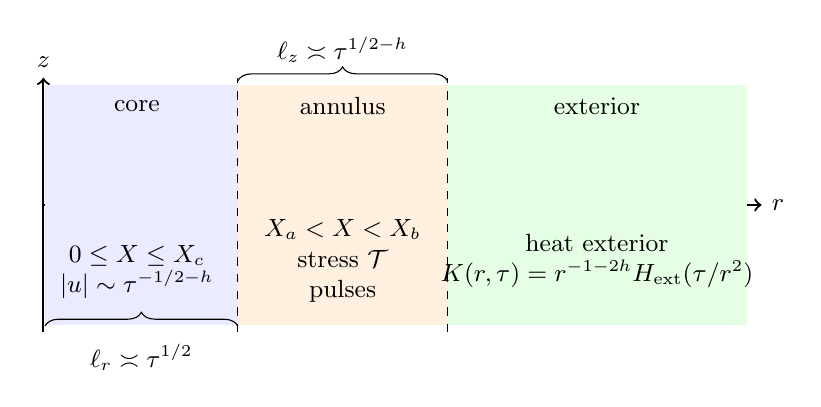
\begin{tikzpicture}[scale=0.95,every node/.style={font=\small}]
  % axis
  \draw[->,thick] (0,0) -- (9.6,0) node[right] {$r$};
  \draw[->,thick] (0,-1.7) -- (0,1.7) node[above] {$z$};
  % regions as vertical bands
  \fill[blue!8]  (0.02,-1.6) rectangle (2.6,1.6);
  \fill[orange!12] (2.6,-1.6) rectangle (5.4,1.6);
  \fill[green!10] (5.4,-1.6) rectangle (9.4,1.6);
  \draw[dashed] (2.6,-1.7) -- (2.6,1.7);
  \draw[dashed] (5.4,-1.7) -- (5.4,1.7);
  \node at (1.25,1.32) {core};
  \node at (4.0,1.32) {annulus};
  \node at (7.4,1.32) {exterior};
  \node[align=center] at (1.25,-0.9) {$0\le X\le X_c$\\$|u|\sim \tau^{-1/2-h}$};
  \node[align=center] at (4.0,-0.75) {$X_a<X<X_b$\\stress $\mathcal{T}$\\pulses};
  \node[align=center] at (7.4,-0.75) {heat exterior\\$K(r,\tau)=r^{-1-2h}H_{\mathrm{ext}}(\tau/r^2)$};
  \draw[decorate,decoration={brace,amplitude=5pt}] (0.02,-1.62) -- (2.6,-1.62) node[midway,below=3pt] {$\ell_r\asymp\tau^{1/2}$};
  \draw[decorate,decoration={brace,amplitude=5pt}] (2.6,1.66) -- (5.4,1.66) node[midway,above=3pt] {$\ell_z\asymp\tau^{1/2-h}$};
\end{tikzpicture}
\end{center}

\begin{enumerate}[label=(\roman*)]
  \item \textbf{Core.} An axisymmetric field whose azimuthal and axial components grow like
        $\tau^{-1/2-h}$ while the radial component grows only like $\tau^{-1/2}$. The core
        is slender: radial scale $\tau^{1/2}$, axial scale $\tau^{1/2-h}$. It solves its
        own leading profile equations exactly, by construction: the profiles $E,U,V_0,\Pi$
        are chosen to satisfy the leading azimuthal and axial balances with radial
        viscosity retained and axial viscosity discarded.
  \item \textbf{Annulus.} Where the core is joined to the exterior, the joining error is
        not smooth in $\tau$. It is written, exactly, as the divergence of a tangential
        stress,
        \[
          R^{(0)}_\theta = -\Bigl(\partial_r+\tfrac2r\Bigr)T_{r\theta},
          \qquad
          R^{(0)}_z = -\Bigl(\partial_r+\tfrac1r\Bigr)T_{rz},
        \]
        supported in an annulus $X_a<X<X_b$ in the similarity variable $X=r^2/2q$.
  \item \textbf{Pulses.} Two families of spatially oscillatory, divergence-free velocities
        are placed in the annulus. Their averaged quadratic fluxes
        $\langle w_r w_\theta\rangle,\langle w_r w_z\rangle$ are made equal to
        $T_{r\theta},T_{rz}$. The families are chosen so that the target stress lies in the
        \emph{interior} of the cone they generate, which is what makes the amplitudes
        positive and the construction stable under perturbation.
  \item \textbf{Exterior.} A purely azimuthal field $K(r,\tau)e_\theta$ solving the radial
        heat equation for the swirl exactly, so that its residual vanishes identically and
        no force is needed there. Its decay rate $r^{-1-2h}$ is what makes the kinetic
        energy of the whole field finite.
\end{enumerate}

The residual of the background plus leading pulses is then not zero but \emph{flat}: every
Cartesian space--time derivative is $O(q^N)$ for every $N$, with $q$ the concentration
scale. Flatness is converted into a smooth force by the localization and extension step.
The single most important structural fact is that the whole construction is a
\emph{finite-stage} object with an \emph{infinite} limit taken at the very end, and that
the limit is taken on vector potentials, not on velocities.

\subsection{The correction cycle}
\label{sec:correction}

Starting from the background plus leading waves, the construction repeats a fixed cycle of
four operations. Writing $u^{[j]},p^{[j]}$ for the fields after $j$ cycles,
\begin{equation}
  u^{[j+1]} = u^{[j]} + \delta u_j,
  \qquad
  p^{[j+1]} = p^{[j]} + \delta p_j,
\end{equation}
the residual changes by the exact identity
\begin{equation}
  \mathcal{R}(u^{[j+1]},p^{[j+1]}) = \mathcal{R}(u^{[j]},p^{[j]})
   + L_{u^{[j]}}(\delta u_j,\delta p_j) + \nabla\cdot(\delta u_j\otimes\delta u_j),
  \label{eq:increment}
\end{equation}
where $L_v$ is the linearization of $\mathcal{R}$ at $v$. The four operations are: solve the
inhomogeneous amplitude equations on the supported angular modes; add signed amplitude
increments whose cross-covariance with the leading pulses supplies a prescribed correction
to the mean stress; correct the angularly averaged residual by inverting the auxiliary-time
derivative; and solve five radial moment equations that keep the pressure and the two
tangential momentum fluxes consistent across the annulus. Each cycle improves a
\emph{residual exponent} $\sigma_j$:
\begin{equation}
  \sigma_0=\tfrac15,\qquad \sigma_{j+1}=\sigma_j+\tfrac1{10},
  \qquad \sigma_j \longrightarrow \infty .
  \label{eq:sigma}
\end{equation}
The exponent arithmetic---which powers of $q$, $S_*=\ell^2$ and the logarithmic edge
weights survive each of the four operations---is isolated in
\file{NavierStokes/ExponentLedger.lean}, a file with no analysis in it at all: it checks the
bookkeeping of \eqref{eq:sigma} against the manuscript's Proposition~10.3, conditionally on
the estimates being valid. This separation is one of the more useful things the
formalization does: the part of the argument that is pure arithmetic is a Lean file about
real numbers, and the part that is analysis is a Lean file about PDEs, and neither can hide
a mistake in the other.

\subsection{Summation, localization and the force}
\label{sec:summation}

The corrections are summed with cutoffs on their \emph{vector potentials}: at stage $j$ one
multiplies the potential $A_j$ and the pressure increment $p_j$ by a cutoff that equals one
on a neighbourhood of the singular point and whose support shrinks with $j$, and then takes
the curl. Taking the curl after multiplication is what keeps incompressibility exact at
every stage. The cutoff losses are controlled because the stage-$j$ estimates lose a power
of $q$ that depends on the derivative order but not on $j$.

After summation one has a local pair $(u_{\mathrm{loc}},p_{\mathrm{loc}})$ on
$\{\tau>0,\ q<q_*\}$ with a potential representation
\begin{equation}
  u_{\mathrm{loc}} = \nabla\times A + B\,e_\theta,
  \label{eq:potential}
\end{equation}
in which both terms are separately divergence-free and both are smooth in Cartesian
coordinates across the axis. The residual is flat in the sense above, the velocity still
grows along the path $u_\theta(\sqrt{2X_{\mathrm{in}}}\tau,0,1-\tau)\sim\tau^{-1/2-h}$, and
the field agrees with the heat exterior for $X\ge X_{\mathrm{ext}}$.

Localization multiplies $A$, $B$ and $p_{\mathrm{loc}}$ by a spatial cutoff $\chi_x$ and a
time cutoff $\chi_t$, and extends by zero. The residual of the localized field differs from
the localized residual by terms supported in the cutoff transition region, away from the
singular point, where the local fields are smooth up to $\tau=0$; hence the difference
extends smoothly through $t=1$ and can be absorbed into the force. The force is then
$f=\mathcal{R}(u,p)$ for $t<1$, extended smoothly past $t=1$; it is compactly supported in
space and in positive time. Energy and dissipation bounds are proved directly from the
equation for the localized fields (not from the local construction), which is why they hold
globally: the core contributes $\tau^{1/2-3h}$, which is bounded and integrable because
$h<1/6$.

The final comparison step is where the theorem's content as a statement about
\emph{non-existence} comes from: any smooth solution with the same force and zero datum and
uniformly bounded energy must agree with the constructed field on every $[0,T]$, $T<1$, by
uniqueness of smooth solutions, and therefore cannot be bounded on a neighbourhood of
$(0,1)$ along the growth path.

\subsection{Euler: packets, amplification and the limiting datum}
\label{sec:euler-shape}

The Euler construction is a different mechanism, and the Lean development reflects that: it
is an iteration on \emph{solutions}, not on a single oscillatory field. At stage $j$ one has
an exact smooth odd solution $U^{j-1}$ (the \emph{parent}), and one adds a localized
oscillation (a \emph{packet}) together with corrections, obtaining an exact smooth solution
$U^j$ (the \emph{child}) on a shorter horizon. The construction maintains
\begin{equation}
  |\nabla U^j(t_j,0)|\longrightarrow\infty,
  \qquad
  \sum_j \|U^j(0)-U^{j-1}(0)\|_{H^m}<\infty \quad (m\ \text{fixed}),
  \label{eq:euler-iteration}
\end{equation}
so the initial data converge in every Sobolev norm to a smooth compactly supported
divergence-free $u_0$, while the gradients at the target times diverge.

The analytic heart is a single \emph{packet estimate}. In particle coordinates
$a\mapsto X(t,a)$ of the parent flow, with $F=\nabla_aX$, $M=\nabla u$ and $H=\nabla^2p$
evaluated along trajectories, one has
\begin{equation}
  \det F=1,\qquad F_t=MF,\qquad F_{tt}=-HF .
\end{equation}
A packet is a velocity increment of the form
\begin{equation}
  w_{\text{lead}}(t,X(t,\ell y)) = \frac{\ell\alpha}{k}\,\chi_1(y)\,v(t,y)\,f_\delta(km_0\cdot y),
  \label{eq:packet}
\end{equation}
where $m=F^{-T}m_0$ is the transported phase normal, $v$ the transverse velocity
coefficient solving
\begin{equation}
  m_t=-M^{T}m,\qquad v_t=-Mv+2m\,\frac{m\cdot Mv}{|m|^2},\qquad m\cdot v=0,
  \label{eq:transverse}
\end{equation}
and $f_\delta$ is an odd zero-mean profile with $f'_\delta(0)=\delta^{-1}$. Differentiating
\eqref{eq:packet} in space produces the leading rank-one gradient
$\alpha\chi_1 v\otimes m f'_\delta$, independent of the frequency $k$: the frequency buys
smallness of the \emph{velocity} at fixed gradient. The child's central shear is then
$\alpha\delta^{-1}|v||m|$, and choosing $\alpha$ makes it the parent shear of the next
stage. The two structural facts that make the iteration close are (a) that the transverse
equation \eqref{eq:transverse} amplifies $v$ exponentially in the parent shear while viscous
damping is absent (Euler), and (b) that the new frame $(m/|m|,v/|v|,n_2)$ again satisfies the
geometric hypotheses needed to run the construction once more.

Each stage therefore requires: a \emph{history} construction (a displacement boundary value
problem on $[0,t_0]$ that prescribes the initial increment), an \emph{oscillatory expansion}
in powers of $k^{-1}$ whose coefficients are obtained from two linear inverses (a mean
inverse with compactly supported initial velocity, and a transverse inverse), a
\emph{correction} that cancels the remaining residual at every derivative order, and a
\emph{summability} check on the initial increments. The whole of
\file{Euler/EulerProof.lean} (20{,}755 lines) is this argument. The final section of the
development turns the iteration into the statement of Theorem~\ref{thm:euler-quant}: the
limiting datum, the maximal lifespan object, the identification of the norms, and the
divergence of the vorticity integral via Beale--Kato--Majda.

\subsection{What a formalization adds}
\label{sec:adds}

Three things in this development have no counterpart in the source papers, and they are the
ones a reader of a formalization should look at.

\paragraph{Objects instead of ``solutions''.} Both papers say ``let $(u,p)$ be the
constructed field''. The formalization has to name the construction: the selected profile
data, the dyadic band index and its chart scale $Q=2^{-\ell}$, the auxiliary torus
$Y\in\T^2$ used to separate oscillating pulses, the label set $\Gamma$ of wave families, the
reserved logarithmic patches inside the annulus, the finite-stage fields and their
potentials. Each of these is a Lean definition with its own API, and the estimate files are
statements about those objects. \file{NavierStokes/ReservedPatches.lean}, for instance,
introduces four disjoint logarithmic intervals $(-25,-20)$, $(-20,-15)$, $(-14,-9)$,
$(-8,-3)$ in the pulse entrance variable, because the manuscript reserves four disjoint
regions for four different corrections. In a paper this is a parenthetical; in Lean it is a
definition plus proofs of disjointness, and every later estimate has to be shown to live in
the right patch.

\paragraph{Hypotheses as data.} The papers' propositions quantify over ``smooth data
satisfying the smallness conditions''. In Lean these become structures whose fields are the
estimates themselves, with the smallness conditions as explicit inequalities between named
constants, and the propositions become functions from those structures to conclusions. This
is why the development is large: a proposition with eleven hypotheses and four conclusions
in a paper becomes a structure, a theorem, and a dozen projection lemmas, and each of the
dozen must be proved before the theorem can be applied.

\paragraph{Flatness as a predicate.} The notion ``the residual vanishes to every order at
the singular point'' is used throughout the Navier--Stokes construction as a property of
fields, and it is what makes the force smooth. The formalization defines it once, proves it
is preserved by the operations of the cycle (summation, multiplication by cutoffs, taking
curls), and uses preservation, rather than re-deriving flatness at each stage. The reader
who wants to know whether the paper's flatness claims are true can read the preservation
lemmas.
